\documentclass{article}

\usepackage{tikz}
\usepackage{fullpage}
\usepackage{amsmath}
\usepackage{amssymb}

\begin{document}

\title{CS499 Deep Learning Lecture Notes}
\author{Toby Dylan Hocking}

Each section is one 75-minute lecture.

\section{Linear algebra}

Why do we care? In ML we have inputs (e.g. image of a digit) and
outputs (e.g. integer class) and the goal is to learn $f$ which takes
the input and yields the correct output.

Inputs are typically represented by vectors/matrices, e.g. grayscale
image actually $[0,1]^{16 \times 16}$ where 0=white and 1=black.

Ex: email message summarized as bag of words.

Matrix multiplication is used to get ML model predictions.

Scalars, vectors, matrices, tensors.

Sets, function domain and range notation.

Subset of a function returning a matrix $f(\mathbf A)_{i,j}$ means
first apply function $f$ then take row $i$ and column $j$.

Transpose, addition, scalar multiplication, matrix-vector addition
(broadcast a vector to each row), matrix product, element-wise
product, dot product.

Properties: associative, distributive, transpose of product, NOT
commutative in general.

System of linear equations $\mathbf A \mathbf x = \mathbf b$, identity
and inverse. Functions for computing $\mathbf A^{-1}$ primarily useful
in theory, but on computers we should solve for $\mathbf x$ using a
function that considers both $\mathbf A,\mathbf b$ (for numerical
stability/precision).

Norms: L1, L2, max, measure size of vectors.

Quiz: given a matrix $\mathbf A$ and $g(x)=x^T$, what is $g(\mathbf A)_{1,2}$?

\section{Probability distributions}

Why? useful for uncertainty. Very suspicious email should have
probability 0.99 of being spam, borderline suspicious email 0.51.

Two interpretations: rates e.g. coin toss, degree of belief
e.g. doctor diagnosis.

Discrete and continuous random variables. Examples: time to relapse,
blood pressure, spam/not digits, clothing classes, number of classes
attended.

Discrete, countably many values (can be ordered), PMF, prob=1 certain,
prob=0 impossible. Different $p$ notations. Three properties: domain
of $p$, all prob values must be between 0 and 1, and must sum to 1
(normalization).

Diagrams. Plot prob versus state/value.

Continuous, uncountably infinitely many values. Three properties of pdf:
domain = set of possible states, all pdf values are non-negative (no
upper bound), and must integrate to 1. PDF is not prob of specific
value, need to integrate to get finite probability.

Quiz: L1-norm of a given vector.

\section{Distributions for outputs in supervised learning}

Begin by explaining supervised learning, inputs, outputs, function to
learn (which is always real-valued, even when the output is
not). Discuss examples of different inputs/outputs along with class.

Table with three rows (Gaussian, Bernoulli, Poisson) and columns:
output space, link distribution $y\sim p(x|f)$.

Define total likelihood $L(f)$ given all training data. Want to find
$f$ that maximizes the probability.

Argmax = argument that results in optimal function value, max =
optimal function value. Draw gaussian argmax.

Information theory. Likely events = low information content, unlikely
events = high information content, independent events additive (two
coin flips yield twice as much info).

Self-information of an event $I(x) = -\log p(x)$.

Shannon entropy of $X\sim p$: $H(p)=H(X)= E_{X\sim p}[I(X)] =
-E_{X\sim P} [ \log P(X) ]$ is the expected amount of information in
an event $X$ drawn from distribution $p$.

KL divergence is useful for ML, because we can learn by finding a
model that minimizes KL-div with respect to data.

\section{Loss functions and gradient descent}

Derive logistic loss using either maximum likelihood or min
KL-divergence.

Introduce project 1 (gradient descent for logistic regression).

\section{Numerical computation}

Gradient, Jacobian, Hessian.

\section{Learning algorithms}

Task $T$: robot learning to walk, classification, regression,
transcription (sound/image to text), translation, etc.

Performance measure/metric $P$: specific to task, often difficult
choice. Partial credit for complex tasks, e.g. whole sentence vs word
in machine translation.

Experience: supervised data set is a collection of examples, design matrix/label
vector. Other settings: unsupervised, semi-supervised, multi-instance,
reinforcement.

e.g. linear regression, MSE on test set.

Q: project 1 task/perf/exp?

\section{Capacity, overfitting, underfitting}

Goal is generalization, which is accurate prediction on new, unseen
test data. Expected value of error on new input (average over samples
in test set).

Q: how do we minimize test error if we only have train samples? Must
assume train and test are drawn iid from same distribution.

Goal is to have an algo that minimizes train error (avoid
underfitting) and minimizes the gap between train/test error (avoid
overfitting).

Capacity/complexity/size is the ability of a model to fit a wide
variety of functions. Draw train/validation error as a function of
model complexity.

Quiz: L2 regularization overfitting plot.

\section{Cross-validation}

Regularization = techniques to simplify model and avoid overfitting
(my definition), modification to reduce generalization error but not
train error (book definition).

Three examples of regularization parameters: (1) iterations, (2)
penalty, (3) polynomial degree.

Parameter vs hyper-parameter. Hyper: must first be fixed before
running learning algorithm. Regular: values found using learning
algorithm.

How to select the regularization/hyper-parameters? Need held out
validation samples (which are not given to the learning algorithm
which computes parameters).

KFoldCV algo. Input Data D, Algo A, Loss L, folds K. Output validation
error vector.

Quiz: in nearest neighbors, what is the number of neighbors which
results in the most complex model?

\section{Fully connected multi-layer Neural Networks}

Want to learn a real-valued prediction function
$f(x)=f^{(L)}[\cdots f^{(1)}[x] ]\in\mathbb R$ which is the repeated
application of $L$ different functions.

Each function $l\in\{1,\dots, L\}$ is a matrix multiplication followed
by an activation function: $f^{(l)}[z] = \sigma^{(l)}[ W^{(l)} z ]$
where $W^{(l)}\in\mathbb R^{u^{(l)}\times u^{(l-1)}}$ and
$z\in\mathbb R^{u^{(l-1)}}$. The last activation function must return
a real number prediction so it is fixed to the identity:
$\sigma^{(L)}[z]=z$. The other activation functions must be
non-linear, e.g. relative linear units (ReLU) $\sigma(z)=(z)_+$,
logistic/sigmoid $\sigma(z)=1/(1+\exp(-z))$. For binary classification
with inputs $x\in\mathbb R^n$, the overall neural network architecture
is $(u^{(0)}=n, u^{(1)}, \dots, u^{(L-1)}, u^{(L)}=1)$, where
$u^{(1)},\dots, u^{(L)}\in\mathbb Z_+$ are positive integers
(hyper-parmeters that control the number of units in each hidden
layer, and the size of the parameter matrices $W^{(l)}$).

Neural network diagrams show how each hidden unit is computed by
applying the weights to the values of the hidden units at the previous
layer.

We can write the units at each layer as
$h^{(0)},h^{(1)},\dots, h^{(L-1)}, h^{(L)}$ where
$h^{(0)}=x\in\mathbb R^n$ is an input feature vector, and
$h^{(L)}\in\mathbb R$ is the predicted output (real-valued score). For
each layer $l\in \{1, \dots, L\}$ we have:
\begin{equation}
  \label{eq:h_l}
  h_l = f^{(l)}\left[h^{(l-1)}\right] =
  \sigma^{(l)}\left[ W^{(l)} h^{(l-1)} \right].
\end{equation}

Total number of parameters to learn is
$\sum_{l=1}^L u^{(l)} u^{(l-1)}.$ Quiz: how many parameters in a
neural network for $n=10$ inputs/features with one hidden layer with
$u=100$ units?

Stochastic gradient descent with randomly selected observation.

\section{Forward and Back-propagation algorithms}

Stochastic gradient descent with epochs. Need gradient of loss with
respect to weights. To do that we use forward propagation then back
propagation.

Forward propagation is the computation of hidden units
$h^{(1)},\dots,h^{(L)}$ given the inputs $x$ and current parameters
$W^{(1)},\dots,W^{(L)}$. Algorithm pseudocode, for loop over layers
from 1 to $L$.

Back propagation is the computation of gradients given current
parameters and hidden units. Algorithm pseudocode, for loop over
layers from $L$ to 1.

Draw diagrams on board. Global diagram start at the bottom right
with $x=h^{(0)}$, go up left to $a^{(1)}$, keep going up to up left
$a^{(L)}=h^{(L)}=\hat y$, then finally the loss $J$. Local diagram
start at the bottom right with $h^{(l-1)}$, go up left to $a^{(l)}$,
keep going to up left $a^{(l+1)}$.

Scalar chain rule formula to keep in mind when deriving back-prop is
\begin{equation}
  \frac{d J}{d v} = \frac{d J}{d z} \frac{d z}{d v},
\end{equation}
where $v$ is the variable for which we want to compute the gradient
(current node in computation graph), and $z$ is the next node up.

To do SGD we need the gradient of the loss with respect to the weight
matrix (write dimensions):
\begin{eqnarray}
  \nabla_{w_k^{(l)}} J
  &=& \left( \frac{d}{d a_k^{(l)}} J \right)
      \left( \nabla_{w_k^{(l)}} a_k^{(l)} \right) =
      \left( \frac{d}{d a_k^{(l)}} J \right)
      h^{(l-1)}\\
  \nabla_{w^{(l)}} J
  &=& \left(\nabla_{a^{(l)}} J\right)
      \left( h^{(l-1)} \right)^T \label{eq:grad-loss-w}
\end{eqnarray}
Then we compute the gradient of the loss with respect to the hidden
units before activation:
\begin{eqnarray}
  \nabla_{a^{(l)}} J
  &=& \left(\nabla_{h^{(l)}} J\right) \odot
      \label{eq:grad-loss-a}
      \left(\nabla_{a^{(l)}} h^{(l)} \right) \\
  &=& \left(\nabla_{h^{(l)}} J\right) \odot \left(h^{(l)}[1-h^{(l)}]\right).\label{eq:logistic-activation}
\end{eqnarray}
The last equation~(\ref{eq:logistic-activation}) is only valid for the
logistic/sigmoid activation funciton.

Then we compute the gradient of the loss with respect to the hidden
units:
\begin{eqnarray}
  \nabla_{h^{(l)}} J
  &=& \left(\nabla_{a^{(l+1)}} J\right)
      \left(\nabla_{h^{(l)}} a^{(l+1)}\right)\\
  &=& \left(\nabla_{a^{(l+1)}} J\right)
      \left(W^{(l+1)}\right)^T \label{eq:grad-loss-h}
\end{eqnarray}

\begin{figure}
  \centering
  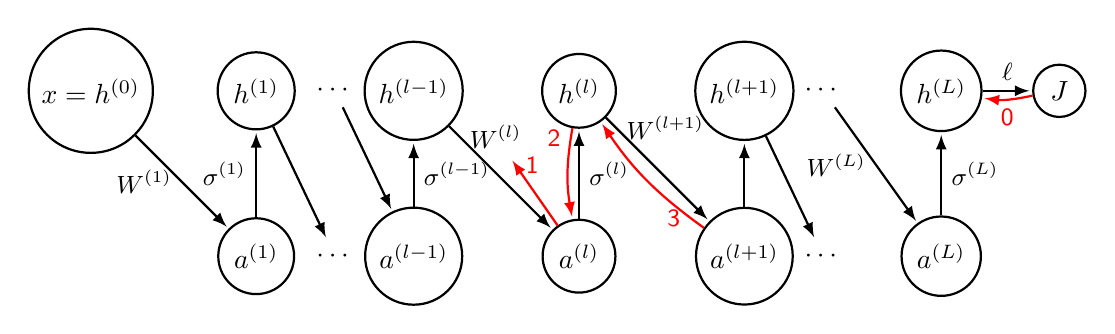
\begin{tikzpicture}[->,>=latex,shorten >=1pt,auto,node distance=2.1cm,
      thick,main node/.style={circle,draw}]

    \node[main node] (h0) {$x = h^{(0)}$};
    \node[main node] (h1) [right of=h0] {$h^{(1)}$};
    \node[main node] (a1) [below of=h1] {$a^{(1)}$};
    \node (a1dots) [right of=a1,node distance=1cm] {$\cdots$};
    \node (h1dots) [right of=h1,node distance=1cm] {$\cdots$};
    \node[main node] (alm1) [right of=a1dots,node distance=1cm] {$a^{(l-1)}$};
    \node[main node] (hlm1) [right of=h1dots,node distance=1cm] {$h^{(l-1)}$};
    \node[main node] (al) [right of=alm1] {$a^{(l)}$};
    \node[main node] (hl) [right of=hlm1] {$h^{(l)}$};
    \node[main node] (alp1) [right of=al] {$a^{(l+1)}$};
    \node[main node] (hlp1) [right of=hl] {$h^{(l+1)}$};
    \node (alp1dots) [right of=alp1,node distance=1cm] {$\cdots$};
    \node (hlp1dots) [right of=hlp1,node distance=1cm] {$\cdots$};
    \node[main node] (aL) [right of=alp1dots,node distance=1.5cm] {$a^{(L)}$};
    \node[main node] (hL) [right of=hlp1dots,node distance=1.5cm] {$h^{(L)}$};
    \node[main node] (J) [right of=hL,node distance=1.5cm] {$J$};

    \path[every node/.style={font=\sffamily\small}]
    %(h0) edge [bend left] node {$c=1, \lambda, m_i\leq m_{i+1}$} (1)
    (h0) edge node [left] {$W^{(1)}$} (a1)
    (a1) edge node [left] {$\sigma^{(1)}$} (h1)
    (h1) edge node [right] {
      %$W^{(2)}$
    } (a1dots)
    (h1dots) edge node [right] {
      %$W^{(l-1)}$
    } (alm1)
    (alm1) edge node [right] {$\sigma^{(l-1)}$} (hlm1)
    (hlm1) edge node [right,name=Wl,pos=0.1] {$W^{(l)}$} (al)
    (al) edge node [right] {$\sigma^{(l)}$} (hl)
    (hl) edge node [right,pos=0.1] {$W^{(l+1)}$} (alp1)
    (alp1) edge node [right] {
      %$\sigma^{(l+1)}$
    } (hlp1)
    (hlp1) edge node [right] {} (alp1dots)
    (hlp1dots) edge node [left] {$W^{(L)}$} (aL)
    (aL) edge node [right] {$\sigma^{(L)}$} (hL)
    (hL) edge node {$\ell$} (J)
    (al) edge [color=red] node [right, pos=0.9] {1} (Wl)
    (hl) edge [bend right=10, color=red] node [left, pos=0.1] {2} (al)
    (alp1) edge [bend left=10, color=red] node [left, pos=0.1] {3} (hl)
    (J) edge [bend left=10, color=red] node {0} (hL)
    ;
  \end{tikzpicture}
  \caption{In black, forward computation graph for a fully connected
    neural network with $L$ matrices of parameters to learn ($L-1$
    hidden layers). Nodes are input/hidden/output units ($a$ before
    activation, $h$ after activation), and edges are computations in
    forward/back propagation ($W$ weight matrix, $\sigma$ activation
    function). In \textcolor{red}{red}, gradient computation rule numbers.}
  \label{fig:forward-back-propagation}
\end{figure}

In Figure~\ref{fig:forward-back-propagation} there are two ways to
interpret the last layer when we are doing binary
classification. If we want the network to output a real-valued
score, then we let the last activation be the identity,
$\sigma^{(L)}(z)=z$, which implies $h^{(L)}=\hat y\in\mathbb R$ can be
used with the logistic loss,
$J =\ell(\hat y, \tilde y) = \log[1+\exp(-\tilde y \hat y)]$, and
labels $\tilde y\in\{-1,1\}$. Equivalently, if we want the network to
output a probability, then we let the last activation function be the
sigmoid, $\sigma^{(L)}(z) = 1/[1+\exp(-z)]$, which implies
$h^{(L)}=\hat p\in[0,1]$ can be used with the binary cross entropy
loss,
\begin{equation}
  \label{eq:binary_cross_entropy_loss}
  J=\ell(\hat p, y) = \log[ 1+ (1/\hat p - 1)^y ] = \begin{cases}
    -\log \hat p & \text{ if } y=1, \\
    -\log (1-\hat p) & \text{ if } y=-1.
  \end{cases}
\end{equation}
Exercise: prove they are equivalent in terms of
gradient computations.

The rules 0--3 for backprop that we discussed in class are shown in
red in Figure~\ref{fig:forward-back-propagation}:
\begin{description}
\item[Rule 0] computes $\nabla_{h^{(L)}} J$, which depends on the
  choice of the loss function $\ell$.
\item[Rule 1] uses (\ref{eq:grad-loss-w}) to compute
  $\nabla_{W^{(l)}} J$ using $\nabla_{a^{(l)}} J$, for any $l\in\{1,\dots,L\}$
\item[Rule 2] uses (\ref{eq:grad-loss-a}) to compute
  $\nabla_{a^{(l)}} J$ using $\nabla_{h^{(l)}} J$, for any $l\in\{1,\dots,L\}$.
\item[Rule 3] uses (\ref{eq:grad-loss-h}) to compute
  $\nabla_{h^{(l)}} J$ using $\nabla_{a^{(l+1)}} J$, for any $l\in\{1,\dots,L-1\}$.
\end{description}
Rule numbering is starting from the parameter of interest, $W^{(l)}$
and working back to the loss $J$ using the chain rule.

\end{document}
